\documentclass[12pt]{amsart}
\usepackage{comment}
\usepackage{ulem}
\usepackage{graphicx}
\usepackage{mathrsfs}
\usepackage{psfrag}
\usepackage{txfonts}

\input{macros.tex}

\begin{document}

\bibliographystyle{plain}

\author{Gregory Crosswhite}
\title{The Astounding Variational Infinite MPS Algorithm}

\maketitle

\tableofcontents

\part*{Phase 1:  Initialization}

\section*{Step 1: Form initial environment}

First, we use Frank Verstraete's algorithm to optimize a system with 10 sites and open boundary conditions, with $\chi=5$.

\begin{center}
\includegraphics[width=5in]{notes-1.pdf}\end{center}

(The purpose of this step is to enlarge the Hilbert space so that it is much bigger than the degrees of freedom in our matrix product state.)

\section*{Step 2: Normalize}

\label{normalize-procedure}

On states 1-5 -- tensors of the form $S_{s\alpha\beta}$, where the index $s$ corresponds to the obsevable and the indices $\alpha$ and $\beta$ are connections to the left and right, i.e.,

\begin{center}
\includegraphics{notes-2.pdf}\end{center}

\noindent we impose the normalization condition:

    \eqn[right-orthog]{\sum_{s\alpha} S_{s\alpha\beta} S_{s\alpha\beta'}^* = \delta_{\beta\beta'}}

That is, we impose the condition that the right index $\beta$ on this tensor is orthonormal, given that the other two indices are orthonormal.  (We may impose this because the $s$ index on all sites is orthonormal, the left index of $S^1$ is orthonormal, and each step orthnormalizes the right on $S^i$ which means that the left index on $S^{i+1}$ is orthonormalized.)  To do this, we perform a singular value decomposition:

    $$S^i_{(s\alpha),\beta} = \sum_{(s'\alpha'),\beta')}U_{(s\alpha)(s'\alpha')} V_{\beta'\beta},$$

\noindent where $U$ and $V$ are unitary and $\Sigma$ is diagonal.  We see that $S^i$ obeys condition \eqref{right-orthog} iff the singular values (i.e., the nonzero elements of the diagonal matrix $\Sigma$) are 1.  Thus, imposing \eqref{right-orthog} is equivalent to setting

    $$S^i_{(s\alpha),\beta} = \sum_{(s'\alpha')=1}^\chi U_{(s\alpha)(s'\alpha')} V_{\beta'\beta}.$$

This process can be represented visually in the following manner:

    
\includegraphics{notes-3.pdf}

Note that this is equivalent to left-multiplying $S^i$ by the matrix,

    \eqn[normalizer]{V^\dagger S^{-1} V.}

Ergo, after setting $S^i$ to the above, we right-multiply $S^{i+1}$ by the inverse of \eqref{normalizer},

    $$V^\dagger S V,$$

\noindent so that at the end of the procedure the state has not been changed.

After sites 1-5 have been normalized, we normalize sites 6-10 (in reverse order) to obey the related condition,

    $$\sum_{s\beta} S_{s\alpha\beta} S_{s\alpha'\beta}^* = \delta_{\alpha\alpha'}.$$

However, we do \emph{not} apply the inverse normalizer to site 5 when normalizing site 6;  this means that we have changed our matrix product state.  Thus, at the end of this process, we obtain a state that looks like,

    \begin{center}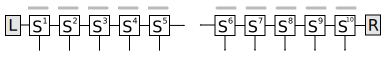
\includegraphics{notes-4.pdf}\end{center}

\noindent with the light-grey arrows indicating the normalization condition imposed on the tensors.

\section*{Step 3:  Build environments}

\label{absorb-multisite-procedure}

Next, we form environments that we can use the calculate the expectations of operators later.  Specifically, for each operator $O$, which we assume has been factored into matrix-product form, we contract the following tensor networks,

    \begin{center}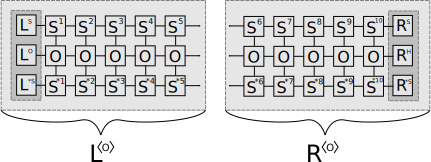
\includegraphics{notes-5.pdf}\end{center}

\noindent to give us left and right environments, $L^{\exp{O}}$ and $R^{\exp{O}}$.  We do this twice to compute environments for $\exp{H}$ and $\exp{I}$ (i.e., the expectation of the Hamiltonian and the normalization.)

We perform the contraction by first multiplying together $L^S$, $L^O$ and $L^{*S}$ as shown in the diagram above, and then absorbing $S^1$, $O$, and $S^{*1}$, then $S^2$, $O$, and $S^{*2}$, etc. until the network is contracted.  (In this way we limit the computational cost to $O(\chi^3)$.)  We adopt a similar strategy for the right environment

\part*{Phase 2: Iteration}

\section*{Step 1:  Prepare for optimization}

At the beginning of this step, we have been given four tensors:  $L^{\exp{H}}$, $R^{\exp{H}}$, $L^{\exp{I}}$, and $R^{\exp{I}}$.  We insert a new site between each of these environments to form a new network as shown:

    \begin{center}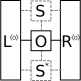
\includegraphics{notes-6.pdf}\textbf{Figure 1}\end{center}

(The site matrix $S$ is grayed in order to indicate that we are deferring our decision of exactly what to put in that spot.)

Contraction of this network is equivalent to computing $\exp{O}$.  We want our new site to minimize the energy -- that is, to minimize the Rayleigh quotient $\exp{H}/\exp{I}$.  Observe that if we were to contract all of the tensors in this network together except for $S$, then we would obtain a matrix, $M^{\exp{O}}$,

    \begin{center}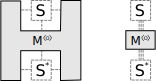
\includegraphics{notes-7.pdf}\end{center}

\noindent such that $\exp{O} = S \cdot M^{\exp{O}} \cdot S^*.$  Thus we see that finding $S$ to minimize our Rayleigh quotient is equivalent to solving the generalized eigenvalue problem,

    $$M^{\exp{H}} S = \lambda M^{\exp{I}} S.$$

We assume that $M^{\exp{I}}$ is sufficiently well conditioned that we can rewrite the above in the form,

    \eqn[evp]{\paren{M^{\exp{I}}}^{-1} M^{\exp{H}} S = \lambda S.}

\noindent We use the ARPACK eigenvalue solver to find the solution to \eqref{evp} with the lowest eigenvalue $\lambda$.  We do not actually calculate $M^{\exp{H}}$ or $M^{\exp{I}}$, however, as this would be inefficient -- a $O(d^2\chi^4)$ operation.  Instead, we observe that for ARPACK, all we really need is the ability to compute the action of $\paren{M^{\exp{I}}}^{-1} M^{\exp{H}}$ on a vector.

Note that multiplying by a matrix $M^{\exp{O}}$ is equivalent to inserting an $S$ (but not $S^*$) into Figure 1 and then contracting all of the tensors together.  Rather than first forming $M^{\exp{O}}$, we can instead leave the network in factored form, and instead absorb first $L^{\exp{O}}$, then $O$, then $R^{\exp{O}}$ into $S$.  The time needed to perform these contractions is $O(2cd\chi^3 + c^3d^2\chi^2)$.

This almost gives us all that we need, save that we also need to compute the action of $\paren{M^{\exp{I}}}^{-1}$.  To do this, we note that this has a special form:  since the identity operator is a tensor product and thus has no ``bonds'', Figure 1 therefore takes the following form:

    \begin{center}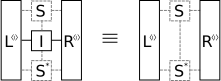
\includegraphics{notes-8.pdf}\end{center}

That is, we see that $L^{\exp{I}}$ and $R^{\exp{I}}$ actually appear in a \emph{tensor product} with respect to each other, and so the inverse is just the tensor product of the inverses.  To find these inverses, we take advantage of the fact that we know that both matrices are Hermitian by construction;  thus, we use a standard Hermitian eigenvalue solver to decompose

    $$L^{\exp{I}} = U_L^\dagger D_L U_L, \quad R^{\exp{I}} = U_R^\dagger D_R U_R,$$

\noindent (an operation which takes $O(\chi^3)$ time) and then obtain the inverse from,

    $$L^{\exp{I}} = U_L^\dagger D_L^{-1} U_L, \quad R^{\exp{I}} = U_R^\dagger D_R^{-1} U_R,$$

\noindent which is also an $O(\chi^3)$ operation.

At the end of the day, we see that computing $\paren{M^{\exp{I}}}^{-1} M^{\exp{H}}S$ is equivalent to contracting the tensor network,

    \begin{center}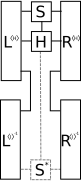
\includegraphics{notes-9.pdf}\end{center}

\noindent which, as before, we perform by first absorbing $L^{\exp{H}}$, then $\paren{L^{\exp{I}}}^{-1}$, etc., so that the entire operation has time complexity $O(cd\chi^3 + c^3d^2\chi^2)$.

\section*{Step 2:  Perform optimization}

We run ARPACK with the following information:

\begin{itemize}
\item A routine to perform matrix-vector multiplication, as described in the previous section
\item The result from the last run of ARPACK to be used as an initial guess (if available)
\item Relative tolerance is $10^{-8}$.
\end{itemize}

The result is a site matrix $S$ which should minimize the energy.

(Sanity checks are performed to make sure that the solution is valid -- i.e., that the solution when plugged into the tensor network gives the same energy as that reported by the eigenvalue solver, that the energy should not have a significant ($>10^{-10}$) imaginary part, etc.)

\section*{Step 3: Normalize and absorb}

Now we want to take our new site and absorb it into the environment.  At each step the site is absorbed into a different side -- i.e., if in the last iteration step we absorbed it into the left then in the next we should absorb it into the right.  Before absorbtion, we normalize it;  if we are absorbing into the left environment, we have to normalize it to the right (i.e., so that it satisfied condition \eqref{right-orthog}) as described in section \ref{normalize-procedure};  if we are absorbing into the right environment, then we have to normalize to the left (i.e., using the other condition).

To absorb, we perform the same process as in section \ref{absorb-multisite-procedure}, save that we only absorb one site into each of the environments.

Normalization is an $O(d^2\chi^3)$ operation (the complexity required to perform the singular value decomposition) and absorbtion is $O(c^2d^2\chi^2 + cd\chi^3)$.

We call the normalized site $\tilde S$ to distinguish it from the unnormalized site $S$ which was obtained from ARPACK.  We feed the unnormalized $S$ into ARPACK in the next iteration, and not $\tilde S$.

Also, when normalizing the site matrix one needs to be careful not to accidently introduce a random phase;  the procedure described in \ref{normalize-procedure} does this, but if one adopts another procedure one must take this into account.

\section*{Step 4: Increase $\chi$}

At this point, we might want to increase $\chi$.  (We could do this, say, once every thousand iterations, or every time some convergence criteria is met.)  To do this, we effectively just absorb a random isometric tensor $U$ and its conjugate into our environments to increase their $\chi$ dimension.

You also need to conjugate the (unnormalized) site matrix $S$ obtained in this iteration about $U$ so that we have something useful to feed into the ARPACK in the next iteration.

\part*{Phase 3:  Compute Expectations}

At some point, we will want to take our site matrix and use to compute the expectation of an operator.  Assuming that we have converged to a translationally invariant site matrix, which we get from the normalized $\tilde S$ in our iteration.  The expectation value $\exp{O^1 O^2}$ where $O^1$ and $O^2$ are local is given by the ratio of the following infinite tensor contractions:

    \begin{center}
\includegraphics{notes-10.pdf}\end{center}

Assuming finite boundary effects, the boundary on the matrix product state will not matter in the finite limit.  In particular, as a result it should be the case that the repeated action of the matrix

    \begin{center}
\includegraphics{notes-11.pdf}\end{center}

\noindent on any (left or right) vector will converge.  This gives us the (left and right) effective infinite environment;  that is, given left and right eigenvectors of this matrix corresponding to the greatest eigenvalue, we can rewrite our quotient in the form,

    \begin{center}
\includegraphics{notes-12.pdf}\end{center}

Finding the $L$ and $R$ eigenvectors is an $O(d^2\chi^3)$ operation as long as we supply ARPACK with a matrix-vector product routine.

\end{document}
